%%%%%%%%%%%%%%%%%%%%%%%%%%%%%%%%%%%%%%%%%%%%%%%%%%%%%%%%%%%%%%%%%%%%%%%%%%%%%%
\section{Simulation of the $\pi+ \to e^+ \nu $ signal }

{\red Briefly Describe the multistage simulation - standard Mu2e scheme
  \begin{itemize}
  \item
    first: simulation of the pion beam, 500x500,000 POT each
  \item
    then - simulation of the $\pi^+ \to e^+ \nu$ decays in the detector
  \end{itemize}
}

\begin{tabularx}{1.0\textwidth} {|X|c|c|c|c|c|}  %
% \begin{tabular}{1.0\textwidth} {|l|l|}  %
  \hline
  Dataset             & degrader thickness & N(ST)       & N(DEG stops) & sum W ST  & sum W(deg)  \\
                      & (mm)               &             &              &           &             \\
  \hline                                                                                          
  bpip0b0             &  no degrader       &   312616    &     0        &   105.7   &              \\
  \hline                                                                                          
  bpip2b0             &     2              &   84785     &   448131     &   276.6   &   454.7      \\
  \hline                                                                                          
  bpip3b0             &     3              &   50340     &   532767     &  272.7    &   977        \\
  \hline                                                                                        
  bpip4b0             &     4              &   31681     &   583855     &  236      &  1537       \\
  \hline                                                                                          
  bpip5b0             &     5              &   17225     &   617324     &  158.8    &   2070       \\
  \hline
\end{tabularx}

Distributions of the pion stop time for different degrader thicknesses are shown in Figure~\ref{fig:pion_stop_time}.
\begin{figure}[H]
  \begin{tikzpicture}
    \node[anchor=south west,inner sep=0] at (0,0.) {
      % \node[shift={(0 cm,0.cm)},inner sep=0,rotate={90}] at (0,0) {}
      \makebox[\textwidth][c] {
        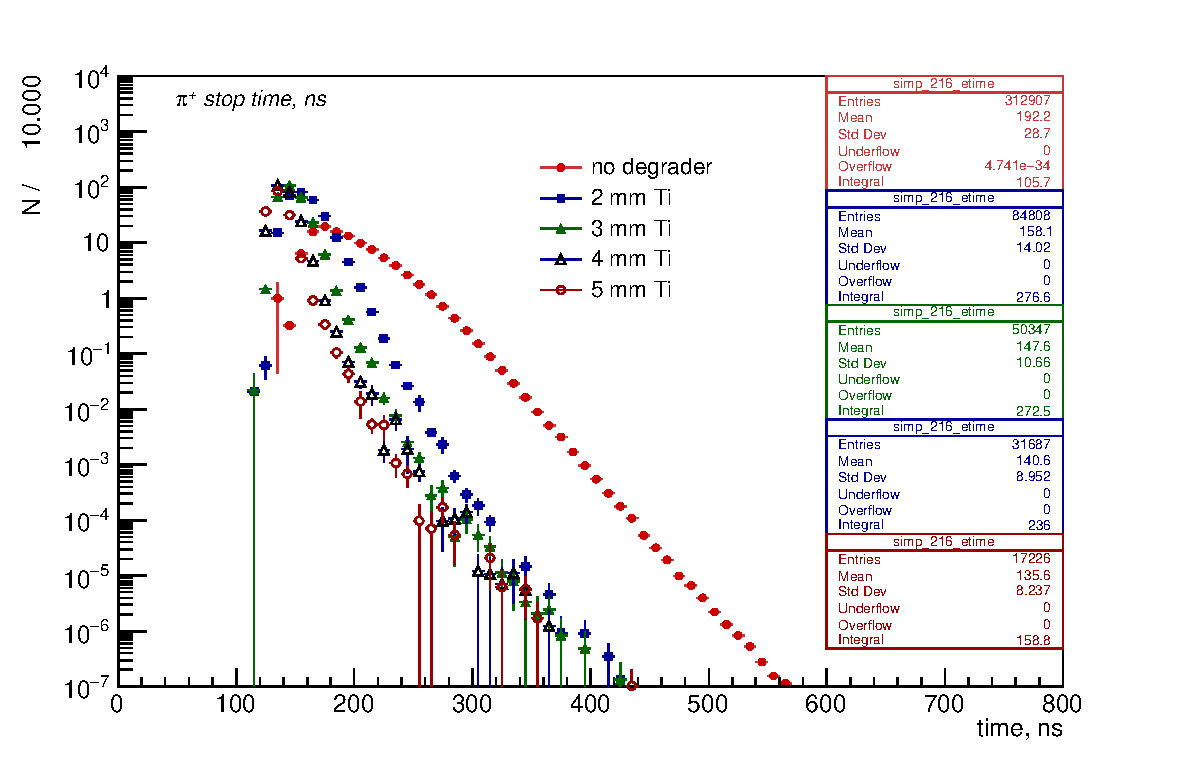
\includegraphics[width=0.55\textwidth]{pdf/figure_02002}
        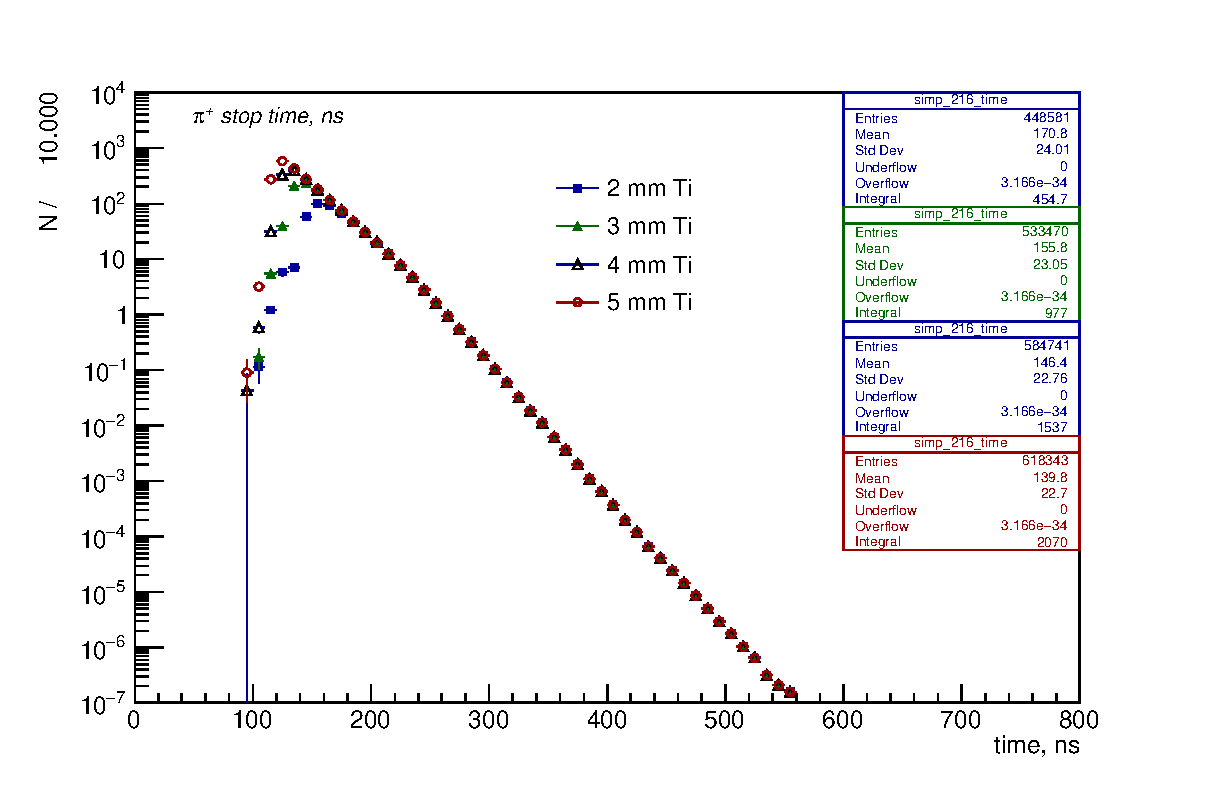
\includegraphics[width=0.55\textwidth]{pdf/figure_02402}
      }
    };
    % \node [text width=8cm, scale=1.0] at (14.5,0.5) {$\mu_B$, expected background mean};
    % \node [text width=8cm, scale=1.0, rotate={90}] at (1.5,7.5) { $S_{D}$, ``discovery'' signal strength  };
  \end{tikzpicture}
  \caption{
    \label{fig:pion_stop_time}
    Distributions of pi stop time for pions stopping in the ST and degrader. The integrals are the sums of weights.
  }
\end{figure}

It is interesting to note that as the degrader thickness increases, teh probability for a pion to stop
in the ST first increases, and after 4mm starts falling down. 
For the pion stops in the degrader, the number continues to increase, and the increase is due
to the stops of faster and faster pions, so additional events accumulate only at early times.

%%%%%%%%%%%%%%%%%%%%%%%%%%%%%%%%%%%%%%%%%%%%%%%%%%%%%%%%%%%%%%%%%%%%%%%%%%%%%% 
\subsection {Pion lifetime: validation}

Weighting events with the pion lifetime - validation plot here

\begin{figure}[H]
  \begin{tikzpicture}
    \node[anchor=south west,inner sep=0] at (0,0.) {
      % \node[shift={(0 cm,0.cm)},inner sep=0,rotate={90}] at (0,0) {}
      \makebox[\textwidth][c] {
        
\includegraphics[width=1.0\textwidth]{pdf/missing_plot}
      }
    };
    \node [text width=8cm, scale=1.0] at (14.5,0.5) {$\mu_B$, expected background mean};
    \node [text width=8cm, scale=1.0, rotate={90}] at (1.5,7.5) { $S_{D}$, ``discovery'' signal strength  };
  \end{tikzpicture}
  \caption{
    \label{fig:pion_lifetime}
  }
\end{figure}

To increase statistics, the pion beam simulation had the charged pion decays turned off.
The survival probability of stopped $\pi^+$'s was stored and used in the analysis
as the event weight.

%%%%%%%%%%%%%%%%%%%%%%%%%%%%%%%%%%%%%%%%%%%%%%%%%%%%%%%%%%%%%%%%%%%%%%%%%%%%%% 
\subsection{Comparison to the BU analysis}

{\red 
\begin{itemize}
\item 
  Compare the signal yield/POT  - should be stable enough.
\item
  BU number : (after all cuts - mu2e-5391 , what are they?): $2.3 x 10^{-12}$ / POT
\end{itemize}
}

